\documentclass[11pt,a4paper]{ctexart}
\usepackage{fontspec}
\setCJKmainfont{Noto Serif CJK SC}
\setCJKsansfont{Noto Sans CJK SC}
\setmainfont{Noto Serif CJK SC}

\usepackage[margin=2.4cm]{geometry}
\usepackage{graphicx}
\usepackage{xcolor}
\usepackage{enumitem}
\usepackage{tcolorbox}
\usepackage{titlesec}
\usepackage{hyperref}
\usepackage{booktabs}
\usepackage{amsmath}

\hypersetup{colorlinks=true, linkcolor=blue!50!black, urlcolor=blue!50!black, citecolor=blue!50!black}

\definecolor{boxblue}{HTML}{4338CA}
\definecolor{boxorange}{HTML}{C2410C}
\definecolor{boxgray}{HTML}{4B5563}

\titleformat{\section}{\Large\bfseries\color{boxblue}}{\thesection}{0.6em}{}
\titleformat{\subsection}{\large\bfseries}{\thesubsection}{0.6em}{}

\newtcolorbox{statusbox}{colback=yellow!8, colframe=orange!70!black, boxrule=0.6pt, arc=2pt, left=8pt, right=8pt, top=6pt, bottom=6pt}
\newtcolorbox{ideabox}[1]{colback=blue!4, colframe=boxblue, boxrule=0.6pt, arc=2pt, left=8pt, right=8pt, top=6pt, bottom=6pt, title=#1, fonttitle=\bfseries}
\newtcolorbox{warnbox}[1]{colback=orange!6, colframe=boxorange, boxrule=0.6pt, arc=2pt, left=8pt, right=8pt, top=6pt, bottom=6pt, title=#1, fonttitle=\bfseries}

\setlist[itemize]{leftmargin=1.4em, itemsep=2pt, topsep=4pt}
\setlist[enumerate]{leftmargin=1.6em, itemsep=2pt, topsep=4pt}

\title{\bfseries 单帧跨具身姿态翻译器 —— 设计草案}
\author{AlphaMotion / Pose Translator 项目组会材料}
\date{\today}

\begin{document}
\maketitle

\begin{statusbox}
\textbf{这份文档的状态：这是一个设计提案，不是定案。}
里面大部分做法都能在别的领域找到先例（借来的），但整体组合起来还没人做过，其中两个关键假设目前只是推理出来的，还没做实验验证（见第 7 节）。汇报的时候请按“提案 + 待验证”来讲，不要讲成“已经跑通”。
\end{statusbox}

% ------------------------------------------------------------
\section{要解决的问题}
% ------------------------------------------------------------

一句话：给一个动作，不管是人做的、动物做的，还是别的什么身体做的，把它\textbf{换到另一个身体上}，而且如果需要，还能\textbf{精确指定某几个关节必须摆到什么位置}。

举两个例子帮助理解要解决的是什么：

\begin{itemize}
    \item \textbf{同一类身体之间}：把人的动作换到人形机器人身上。这种情况下“正确答案”是明确的——人抬手，机器人也应该抬手，可以用现成的经典算法（比如 GMR）先生成一批“标准答案”，拿来当监督信号。
    \item \textbf{完全不同的身体之间}：把老鹰扇翅膀的动作换到人形机器人身上。这种情况下\textbf{没有唯一正确答案}——老鹰的翅膀该对应机器人手臂的哪个部位，这本身就没有标准解。这跟人练“螳螂拳”是一回事：人不是把螳螂的关节角度照抄过来，而是理解螳螂动作里“快、准、勾手发力”这些更抽象的东西，再用人自己的身体重新表达一遍。
\end{itemize}

这两种情况要用不同的方式训练（第 5 节展开），但\textbf{用的是同一个网络，同一套架构}，不是两个模型。

现在业界常用的方法（比如 GMR）是经典的逆运动学（IK）算法，每换一种身体都要人工写一份“对应关系表”。我们想用一个网络替代这个人工过程，而且额外要求：能精确控制个别关节（比如“手必须摸到这个点”），这是经典 IK 工具本来就有的能力，但现有的神经网络方法（下面会提到的几篇论文）基本都没做到。

% ------------------------------------------------------------
\section{整体思路}
% ------------------------------------------------------------

\begin{figure}[h]
    \centering
    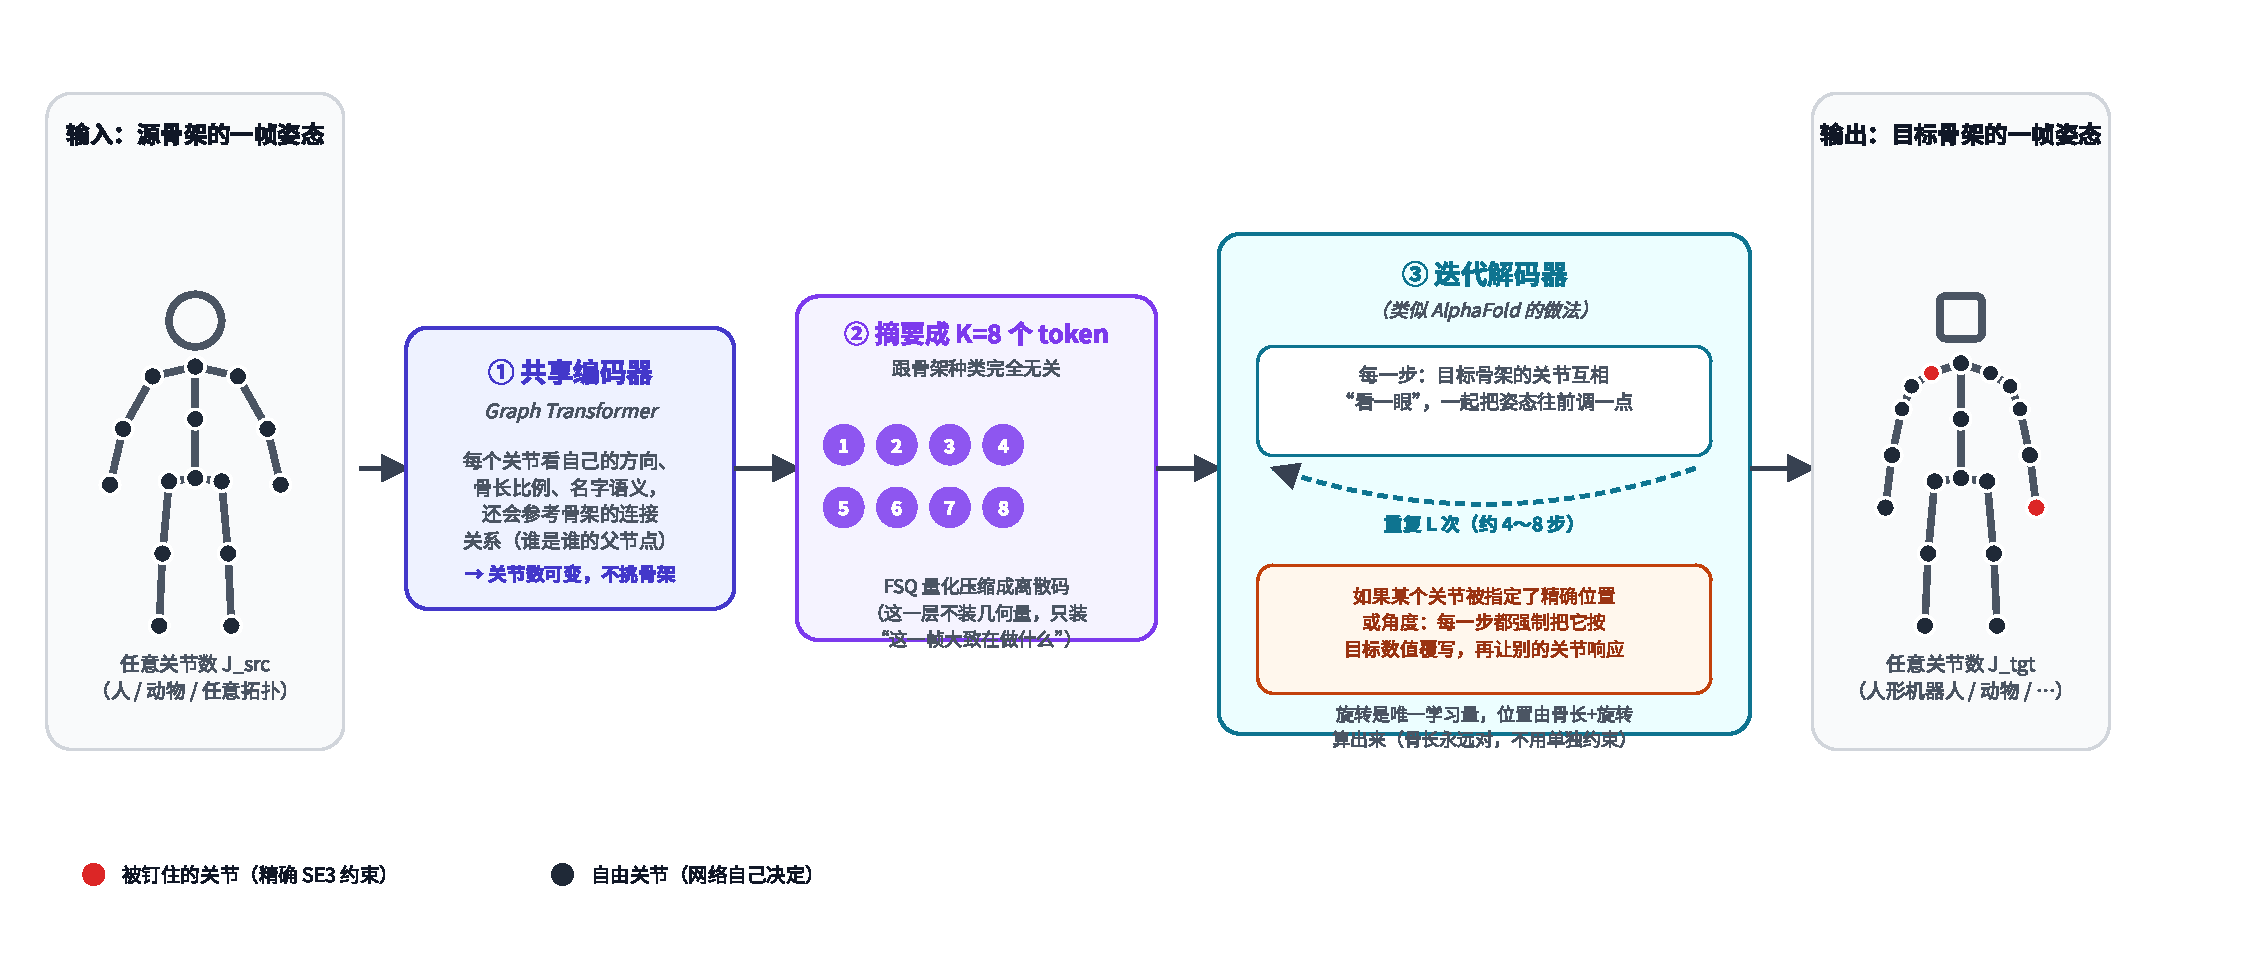
\includegraphics[width=\textwidth]{figures/fig1_pipeline.pdf}
    \caption{整体流程：源骨架 $\to$ 共享编码器 $\to$ K=8 个抽象摘要 $\to$ 迭代解码器（可精确控制）$\to$ 目标骨架}
\end{figure}

流程分三步，全部用同一套参数处理任意骨架，不用为每种身体单独训练：

\begin{enumerate}
    \item \textbf{编码器}：把源骨架的每个关节（不管有多少个）读进来，输出一批特征。这一步只关心“这个关节朝哪个方向、骨头多长、叫什么名字、跟谁相连”，不关心具体是人还是动物。
    \item \textbf{摘要成 8 个抽象 token}：不管源骨架有多少个关节，都压缩成固定的 8 个“摘要”。这 8 个摘要跟骨架种类完全无关，装的是“这一帧大概在做什么动作”这种抽象信息，几何坐标反而不装在这里。
    \item \textbf{迭代解码器}：拿着这 8 个摘要和目标骨架的信息（骨长、关节数、连接关系），一步步“展开”成目标骨架的具体姿态。做法参考了 AlphaFold 预测蛋白质结构的方式：不是一次性算出答案，而是让目标骨架的所有关节反复互相“看一眼”，每看一轮就把姿态往合理的方向调一点，调个几轮（4 到 8 轮）就收敛。这一步也是精确控制生效的地方（第 4 节）。
\end{enumerate}

% ------------------------------------------------------------
\section{两个真正的难点}
% ------------------------------------------------------------

\subsection{难点一：骨架之间的关节对不上}

\begin{figure}[h]
    \centering
    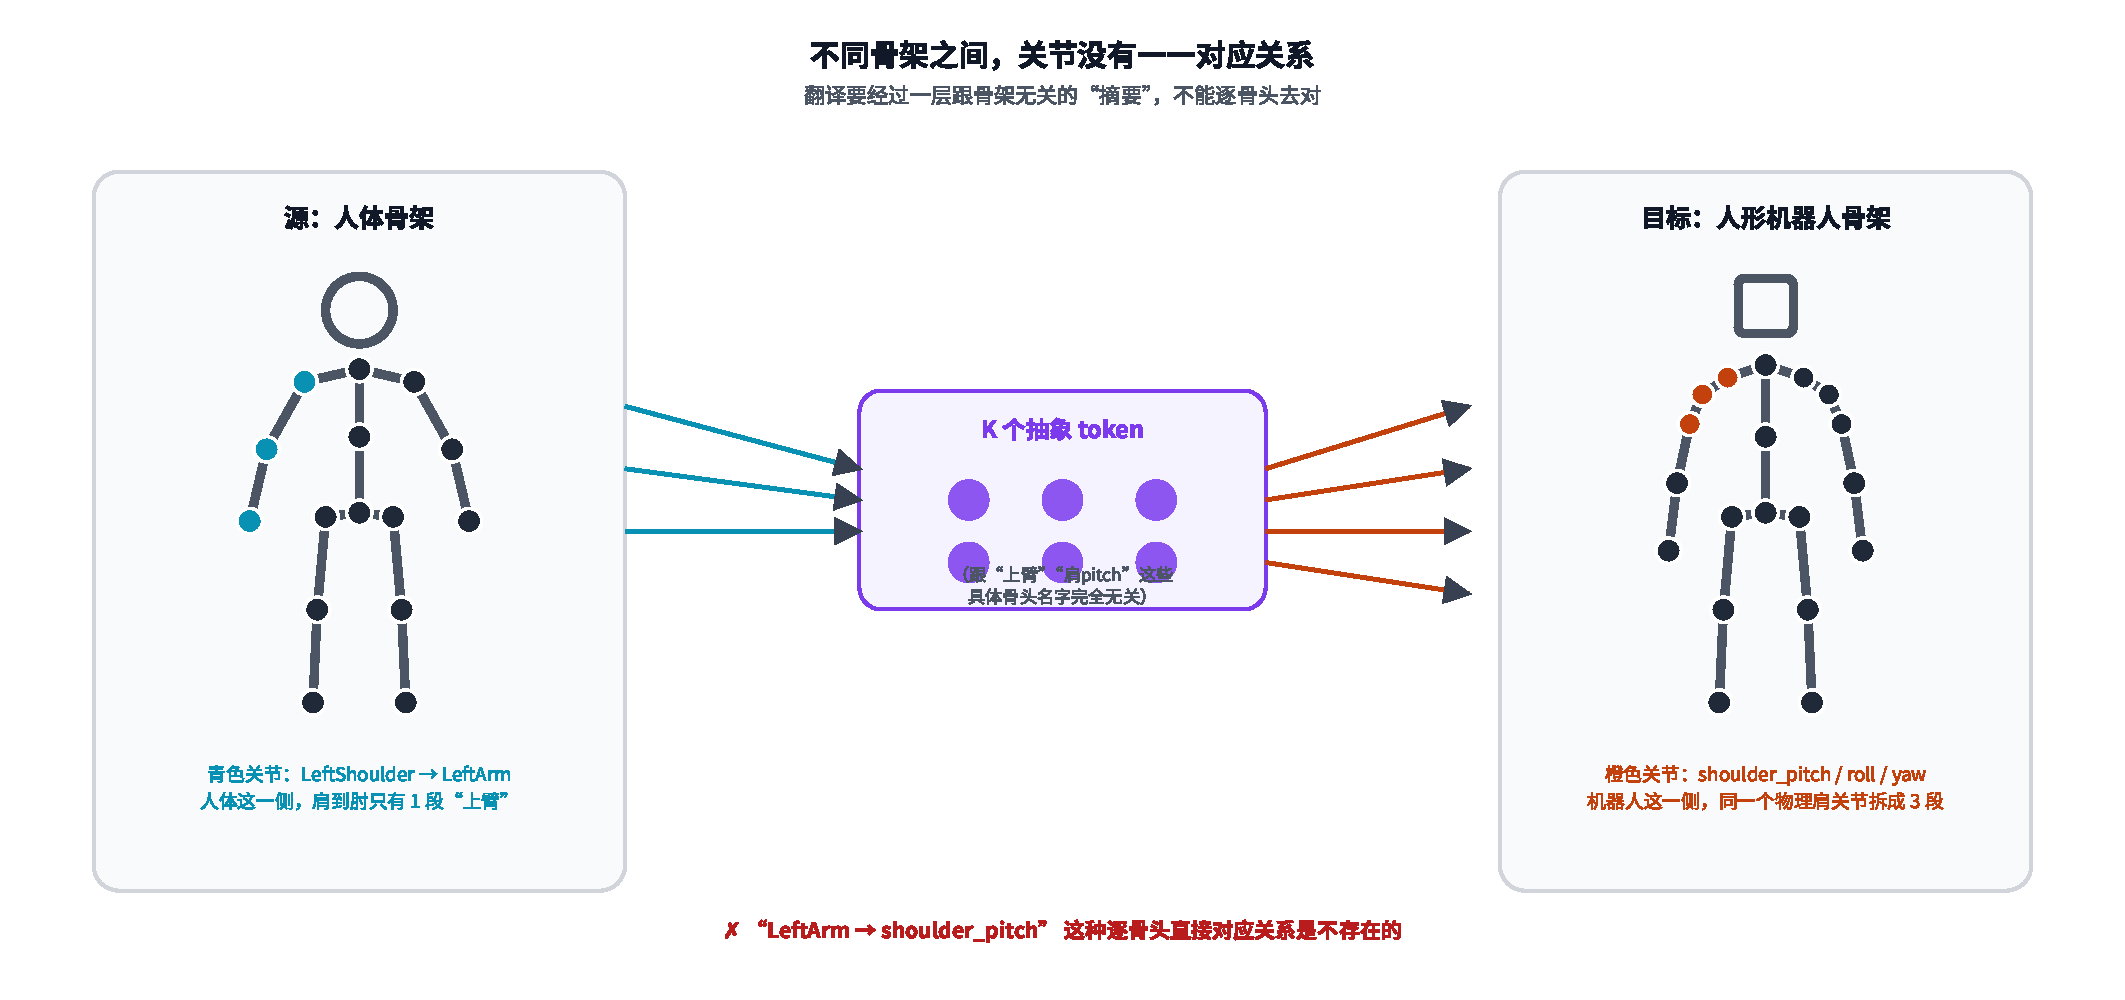
\includegraphics[width=0.92\textwidth]{figures/fig3_cross_topology.pdf}
    \caption{人的“上臂”和机器人的“肩关节三段”不是同一个东西，逐骨头去对应是行不通的}
\end{figure}

我们实际测过：人体骨架里“LeftArm”就是一整段上臂；而人形机器人经常把物理上的一个肩关节拆成三段串联的轴（pitch/roll/yaw）分别转。把人的上臂方向直接抄到机器人的某一段轴上，效果反而比什么都不做还差。

\textbf{结论：不存在“一根骨头对应另一根骨头”这种映射关系。} 这也是为什么这件事必须让网络来学，而不是写一张对应表——网络学的是“整体姿态在表达什么”，展开到目标骨架的哪根骨头上，是网络自己决定的，不是人工指定的。

\subsection{难点二：骨头会不会绕自己转，从位置上完全看不出来}

\begin{figure}[h]
    \centering
    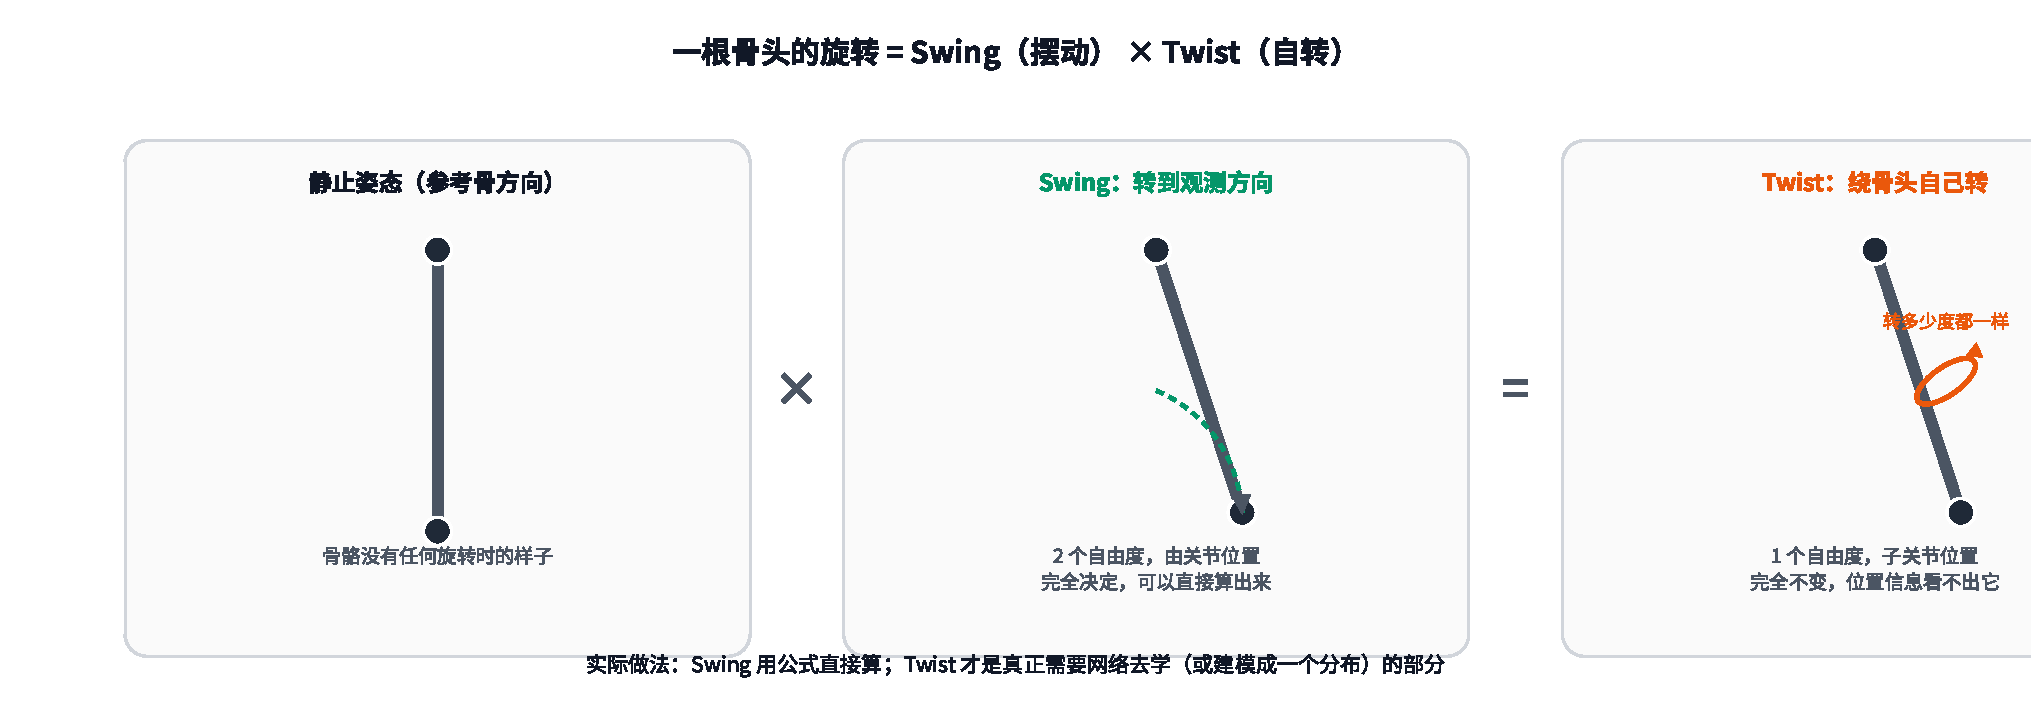
\includegraphics[width=0.92\textwidth]{figures/fig2_swing_twist.pdf}
    \caption{一根骨头的旋转可以拆成两部分：Swing 能算出来，Twist 看不出来}
\end{figure}

一根骨头的旋转其实是两件事叠加：

\begin{itemize}
    \item \textbf{Swing（摆动）}：骨头指向哪个方向。这个可以直接从关节位置算出来，不需要网络猜。
    \item \textbf{Twist（自转）}：骨头绕着自己这根轴转多少度。\textbf{不管转多少度，子关节的位置完全不变}——所以单看位置，这个信息是彻底缺失的，不是网络学得不够好，是数学上就看不出来。
\end{itemize}

做法：Swing 部分用公式直接算，不浪费网络的学习能力；Twist 部分才是真正需要网络处理的地方——如果源动作本身有旋转信息（比如同类身体之间的翻译），就让网络去学；如果源动作没有旋转信息（比如跨物种翻译，本来就没有这个概念），就不逼网络给出一个确定值，而是让它给一个“大概率范围”，避免瞎猜出一个错得离谱的数字。

% ------------------------------------------------------------
\section{怎么做到“精确控制”}
% ------------------------------------------------------------

\begin{figure}[h]
    \centering
    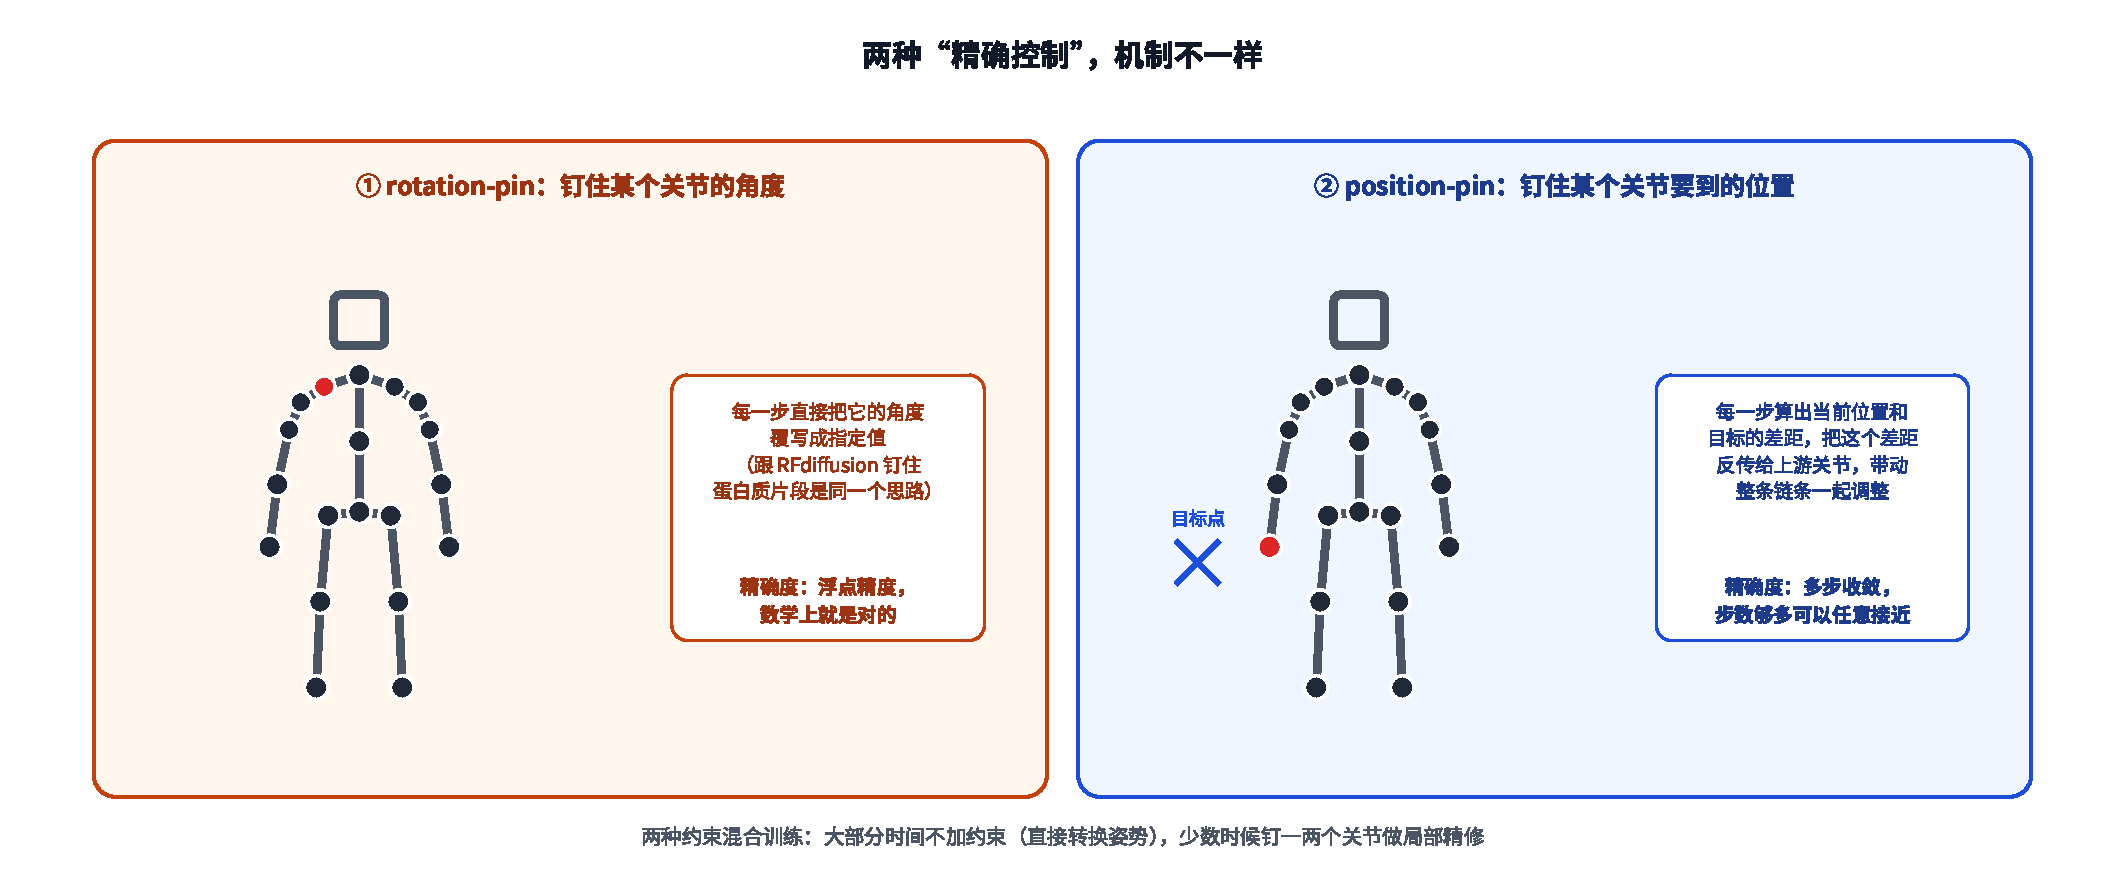
\includegraphics[width=0.92\textwidth]{figures/fig4_constraints.pdf}
    \caption{钉角度和钉位置，机制不一样，精确程度也不一样}
\end{figure}

精确控制分两种情况，机制完全不同：

\begin{description}
    \item[钉角度] 比如“这个关节必须转到 30 度”。做法很简单：解码器每一步迭代完，直接把这个关节的角度\textbf{强制改写}成指定值，再让其它关节根据这个新信息调整自己。这是数学上精确的，不存在误差。
    \item[钉位置] 比如“这只手必须摸到空间里的这个点”。这个更难，因为位置是骨长和好几个关节角度共同决定的，不能直接改写。做法是每一步迭代都算一下“现在的位置离目标还差多少”，把这个差距转换成信号，推动前面那一串关节一起调整角度——这其实就是经典的\textbf{逆运动学（IK）}，只是放进了迭代解码的过程里，迭代的轮数越多，越接近目标。
\end{description}

大部分时候（比如直接把一个动作换到另一个身体上）\textbf{不需要任何约束}，两种机制都不触发，模型自动退化成纯粹的“翻译”。只有需要精修的时候才用得上。训练的时候要让“完全不约束”的情况占大多数，不然网络会偷懒变成只会解约束方程的计算器，忘了怎么看源动作。

% ------------------------------------------------------------
\section{训练怎么分两种情况}
% ------------------------------------------------------------

\begin{ideabox}{同一类身体之间（比如人 $\to$ 人形机器人）}
可以用经典算法（如 GMR）先批量生成一批“标准答案”当监督信号。直接比较网络输出和标准答案的差距去训练，跟普通的监督学习一样。
\end{ideabox}

\begin{ideabox}{完全不同的身体之间（比如老鹰 $\to$ 人形机器人）}
没有标准答案，不能用“跟GT差多少”这种方式训练。改用两类信号：
\begin{itemize}
    \item 生成的动作\textbf{像不像}目标身体自己会做出来的动作——用一个判别器打分，而不是逐点比较坐标
    \item 源动作和生成动作在一个“语义空间”里\textbf{够不够接近}——这个语义空间可以借助动作的文字描述来建立（类似“人在打太极”和“生成的机器人动作也像在打太极”这种语义层面的接近）
\end{itemize}
另外，每种身体自己的动作数据要参与“自己转换成自己”的训练，让网络的抽象摘要真的对这种身体的骨架结构有效，不是靠死记硬背人形骨架蒙混过关。
\end{ideabox}

同一个训练过程里，两类样本混着采样，遇到哪类样本就用哪种损失函数，不是分成两个阶段或者两个模型。

% ------------------------------------------------------------
\section{以后要接时间序列，现在要留好接口}
% ------------------------------------------------------------

这个版本只处理单独一帧，不管时间。但已知一个坑：如果以后把这套解码器逐帧独立地用在一段视频/序列上，容易\textbf{抖}——尤其是上面提到的“看不出来”的 Twist，如果每一帧都独立猜一个数，相邻两帧完全可能给出两个都“合理”但差很远的值，看起来就是关节在原地闪烁或打转。这在做视频姿态估计的领域里是个已知问题，已经有一些常见的补救办法（比如单独训练一个轻量的时序平滑模块，专门修这种抖动）。

这个版本暂时不处理这个问题，但设计的时候要注意：不要把“每一步都从头开始猜”这种假设写死进架构里，以后至少要能做到“参考上一帧的结果去初始化这一帧”，方便后续扩展。

% ------------------------------------------------------------
\section{还没验证、需要做实验的地方}
% ------------------------------------------------------------

\begin{warnbox}{这两件事目前只有推理，没有实验支撑，是这份提案里最不确定的部分}
\begin{enumerate}
    \item \textbf{8 个抽象 token 到底需要压缩到多细}：之前在另一个相关项目里，对“骨头方向向量”做过一次类似的压缩实验，发现压缩比特数越高、浪费的比例反而越大。但这次要压缩的是“抽象摘要向量”，不是方向向量，形状完全不同，旧结论不能直接套用，需要重新做一轮实验：先估计这批数据到底有多少种“本质上不同的动作”，再实际测不同压缩程度下，还原出来的动作精不精确。
    \item \textbf{逐帧独立解码，会不会真的抖}：需要专门构造一个“骨头自转角度完全没有线索”的测试场景，实际跑一遍逐帧独立解码，量一下抖动到底有多大，再看“参考上一帧结果初始化”这种简单办法能不能把抖动压住。
\end{enumerate}
这两个实验都是几天量级能跑完的小实验，建议在往下写完整实现之前先跑完，免得方向错了返工代价更大。
\end{warnbox}

% ------------------------------------------------------------
\section{这个设计参考了哪些论文}
% ------------------------------------------------------------

不是凭空设计的，每一块基本都能在下面某一篇论文里找到对应的先例，只是没有人把这些拼在一起过：

\begin{itemize}[leftmargin=1.6em]
    \item \textbf{跨骨架摘要成固定数量 token}：SAMoR (arXiv:2607.02148)、PALUM (arXiv:2601.07272)
    \item \textbf{旋转参考锚点（不同骨架的旋转怎么变得可比较）}：MoCapAnything V2 (arXiv:2604.28130)
    \item \textbf{Swing/Twist 分解}：HybrIK (arXiv:2011.14672)、NIKI (arXiv:2305.08590)
    \item \textbf{迭代式精确坐标预测（IPA）}：AlphaFold2 (Jumper et al., \textit{Nature} 2021)
    \item \textbf{钉住部分结果、生成其余部分}：RFdiffusion motif scaffolding (Watson et al., \textit{Nature} 2023)；SE(3) 流匹配下的两种钉法：Improved Motif-Scaffolding (arXiv:2401.04082)
    \item \textbf{推理时用梯度引导实现空间约束}：OmniControl (arXiv:2310.08580)
    \item \textbf{没有标准答案时怎么训练跨物种迁移}：SATA (arXiv:2605.27055)、ACE (ACM SIGGRAPH Asia 2023)
    \item \textbf{逐帧独立估计会抖，怎么修}：SmoothNet (arXiv:2112.13715)
    \item \textbf{旋转的神经网络友好表示}：Zhou et al., ``On the Continuity of Rotation Representations in Neural Networks'' (CVPR 2019)
    \item \textbf{跨骨架网络结构的早期工作}：Aberman et al., ``Skeleton-Aware Networks for Deep Motion Retargeting'' (arXiv:2005.05732)
\end{itemize}

\end{document}
